\documentclass[11pt]{article}
\usepackage[utf8]{inputenc}
\usepackage{mathtools}
\usepackage{empheq}
\usepackage{graphicx}
\usepackage{amssymb}
\usepackage{titlesec}
\usepackage{systeme}

\setcounter{secnumdepth}{4}

\title{Physique Oscillation Harmonique}
\author{Vanden Driessche Théo}

\date{November 2017}


\usepackage{geometry}
 \geometry{
 a4paper,
 total={170mm,257mm},
 left=20mm,
 top=20mm,
 }
\graphicspath{ {images/} }

\begin{document}

\maketitle

\newpage
\section{Phènomènes périodiques}
\subsection{Définitions}
-Un oscillateur est un objet décrivant un mouvement de va-et-vient de part et d'autre d'une position d'équilibre.\\
-L'élongation y d'un point P est la valeur algébrique de l'écart de P par rapport à la position d'équilibre O.

\subsection{Caractéristiques d'une oscillation}
\subsubsection{Période et fréquence}
\begin{align*}
        f&=\dfrac{1}{T} \Longleftrightarrow &T=\dfrac{1}{f} \\
        f& \Rightarrow Hz &T \Rightarrow s   
\end{align*}

\section{Mouvements Harmoniques}
\subsection{Définition}
Un mouvement harmonique est un mouvement d'oscillation dont la représentation graphique de l'élongation en fonction du temps est une sinusoïde.\\

\subsection{Amplitude}
-L'amplitude est l'écart maximal par rapport à la position d'équilibre c'est à dire l'élongation maximale. On la note A l'unité SI est le mètre (m).\\
L'amplitude correspond à la position maximale $ A = y_{(t)max}$\\
La période T coresspond au temps mis par oscillation.\\
La frequence f correspond au nombre d'oscillation par seconde.
\begin{center}
    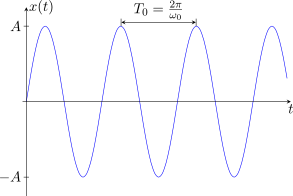
\includegraphics{oscillateur_harmonique.png}
\end{center}

\newpage
\subsection{Étude mathématique}
Supposons d'abord que la position $M_{0}$ du point M à l'instant t=0 se situe sur CX, à droite de C. L'angle $\alpha$ formé par CX et CM, qui vaut 0 à l'instant t = 0, augmente régulièrement puisque M tourne à vitesse constante.\\
La vitesse angulaire est l'angle balayé par CM par unité de temps. La notation est $\omega$. L'unité SI est le radian/seconde (rad/s).\\
$$\omega = \dfrac{\alpha}{t} \text{ ou } \alpha=\omega \cdot t$$
Projetons le mouvement de M sur un axe vertical OY. La projection P de M décrit un mouvement d'oscillation de part et d'autre de C. La valeur algébrique de CP est l'élongation. On voit que $-A \leqslant y \leqslant A $\\
La période T de P est la durée d'une oscillation complète, ce qui correspond à un tour complet. Par consequent, $\alpha _{(T)}=2\pi$.\\
Or $\alpha=\omega \cdot t$ donc $\alpha _{(T)}=\omega \cdot T = 2\pi$\\
$y_{(t)} = CP = QM = CM \cdot sin(\alpha) = A \cdot sin(\omega t)$
%\begin{gather}
 %   y_{(t)} =A\cdot sin(\alpha _{(t)}) = A\cdot sin(\omega t)    \\
  %  \omega = 2\pi f = \dfrac{2\pi}{T}
%\end{gather}

\begin{center}
    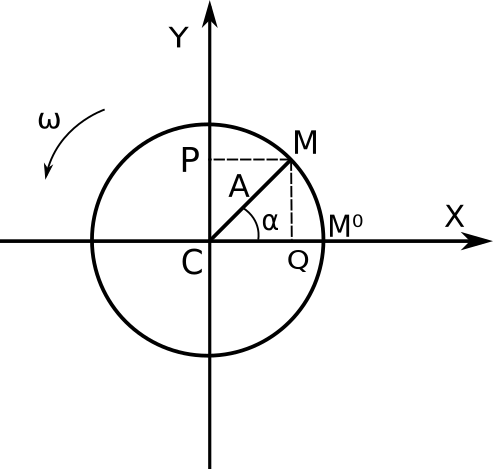
\includegraphics[scale=0.5]{Fig1_8.png}
\end{center}
\section{Dynamique}
\subsection{}

\begin{empheq}[left=\empheqlbrace]{align}
\sum F & =ma \\
 a & = -\omega^2 y 
\end{empheq}
\begin{align*}
\Rightarrow \sum F & = -m\omega ^2 y \\
\text{ Où }  -m\omega ^2 & \text{ est constant.}
\end{align*}

\subsection{Rappel: Loi d'Hooke}
\begin{align}
    F = -kx
\end{align}
Toute force de ce type provoque un mouvement d'oscillation harmonique
par consequent:
la période peut être déduite de la relation
$$\omega = \sqrt{\dfrac{k}{m}} $$
$$T = 2 \pi \sqrt{\dfrac{m}{k}}$$
\subsection{Le pendule simple}


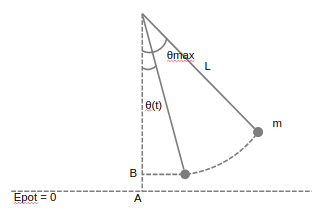
\includegraphics{testSimplePendulum.png}

Que peut faire varier la période d'un pendule simple? \\
-Son Energie de départ (E) \\
-La longeur de la corde (L) \\
-la pesanteur (g) \\

\subsubsection{Epot}
\begin{equation}
\begin{split}
    E_{tot} & = E_{pot} + E_{cin} \\
    & = mg|AB| \\
    & = mg(L-Lcos(\theta_{(t)})) \\
    & = mgL(1-cos(\theta_{(t)}))
\end{split}
\end{equation}

\subsubsection{Ecin}
\begin{align*}
E_{cin} & = \dfrac{mv^2}{2}  & v = v_{ang}L \\
&     & = \theta ' _{(t)}L & \text{ la dérivée de l'angle décrit} \\
& = \dfrac{m(\theta ' _{(t)} L)^2}{2}\\
\end{align*}

\subsubsection{Etot}
Energie totale est constante (Frottements négligeables). \\
Donc la variation d'Etot = 0. Par conséquent, sa dérivée vaux zéro.\\
$$(E_{tot})'=0$$ \\
Nous pouvons donc dire:
\begin{equation}
\begin{split}
    (E_{pot})'  & = (E_{cin} + E_{pot})' \\
    0 & = \Bigg( \dfrac{m(\theta_{(t)}' L)^2}{2} + mgL\Big(1-cos(\theta_{(t)})\Big)\Bigg)' \\
    & = \Bigg( \dfrac{m(\theta_{(t)})'^2 L^2}{2} + mgL\Big(1-cos(\theta_{(t)})\Big)\Bigg)' \\
    & = \dfrac{2}{2}mL^2 \theta_{(t)} ' \theta_{(t)}'' + mgLsin(\theta_{(t)})\theta_{(t)}' \\
    & = L \theta_{(t)}'' + y\cdot sin(\theta_{(t)}) \\
    \theta_{(t)}'' & =\dfrac{ -y\cdot sin(\theta_{(t)})}{L}
\end{split}
\end{equation}


\begin{equation}
\begin{split}
\text{Si, } \theta < \dfrac{\pi}{6} \text{ ,on a } & sin(\theta) \cong \theta \text{ alors,}\\
\end{split}
\end{equation}
$$\theta_{(t)}'' + \dfrac{g}{L} \theta_{(t)} = 0$$ \\
Une solution de cette équation différentielle, où l'on suppose que $\omega^2 = \dfrac{g}{L}$,  est: \\
$$\theta_{(t)} = \theta_{max} sin(\omega t + \varphi)$$\\
\begin{align*}
    \omega^2 & = \dfrac{g}{L} 
    & \omega = \sqrt{\dfrac{g}{L}}&
    &\dfrac{2\pi}{T}  = \sqrt{\dfrac{g}{L}}\\
    T & = \dfrac{2\pi \sqrt{\dfrac{g}{L}}L}{2}
    & T = 2\pi \sqrt{\dfrac{L}{g}} &
\end{align*}

\subsection{Energie}
\subsubsection{Énergie cinétique}
\begin{equation}
\begin{split}
    E_{cin}  = \dfrac{mv^2}{2} & = \dfrac{m\Big(\omega A \cdot cos(\omega t+ \varphi)\Big)^2}{2} \\
    & =\dfrac{ m\omega^2 A^2 cos^2(\omega t+ \varphi)}{2} \text{ Par l'égalité fondamentale: } \\
    & = \dfrac{ m\omega^2 A^2 \Big(1-sin^2(\omega t+ \varphi)\Big)}{2} \\
    & =\dfrac{m\omega^2\Big(A^2-A^2sin^2(\omega t+ \varphi)\Big)}{2} \\
    & =\dfrac{m\omega^2(A^2-y_{(t)}^2)}{2} \\
    & = \dfrac{k(A^2-y_{(t)}^2)}{2}
\end{split}
\end{equation}
\subsubsection{Énergie totale}
 L'énergie totale est égale à l'énergie cinetique lorsque $y_{(t)}=0$ \\
 \begin{equation}
     \begin{split}
         E_{tot} & = E_{cinMax}\\
        & = \frac{kA^2}{2}
     \end{split}
 \end{equation}
\subsubsection{Énergie potentielle élastique}
Par définition, $E_{pot} = E_{tot}-E_{cin}$ \\
\begin{equation}
    \begin{split}
        E_{pot} & = E_{tot}-E_{cin} \\
        & = \frac{kA^2}{2} - \dfrac{k(A^2-y_{(t)}^2)}{2} \\
        & = \frac{k(A^2-A^2+y_{(t)}^2)}{2} \\
        & = \frac{ky_{(t)}^2}{2}
    \end{split}
\end{equation}

\subsection{Oscillations amorties}
Il existe des forces dissipatives, $E_{mec}$ n'est pas conservée. Ceci entraine une diminution de l'Amplitude (A) au fil du temps (t).\\
En general, $F_{dissip}=\gamma \cdot v$ où $\gamma$ est une constante d'amortissement.
\section{Résonance}
\subsection{Définitions}
\begin{itemize}
    \item lorsque le transfet d'énergie est maximum, on dit qu'il y a résonance.
\end{itemize}
\subsection{Conclusions}
\begin{enumerate}
    \item Il y a résonance lorsque la fréquence propre du résonateur est égale à la fréquence propre de l'excitateur
    \item Le transfert d'énergie a donc un caractère sélectif: le résonateur absorbe de façon préférentielle à sa fréquence propre.
\end{enumerate}
\subsection{Application mathématique}
\begin{equation}
    k= \dfrac{F_p}{x}=\dfrac{m\cdot g}{x}
\end{equation}

\section{Ondes progressives}
\subsection{Définition}
Transfert d'énérgie sans transfert de matère.
\subsection{Types}
\begin{itemize}
    \item Ondes transversales
    \item Ondes longitudinales
\end{itemize}
\subsection{Vitesse}
Dépend du milieu et de la nature du signal
\subsection{Ondes sinusoïdales entretenues}
\subsubsection{Longueur d'onde}
\begin{equation}
    \lambda = v \cdot T = \dfrac{v}{f}
\end{equation}
Distance minimale entre 2 points en concordance de phase.
\subsubsection{Études mathématiques}
Prenons l'équation en fonction du temps de l'élongation de S (la source) et supposons que $\varphi = 0$
\begin{equation}
    y_{S(t)}= A \cdot sin(\omega t)
\end{equation}

\begin{center}
    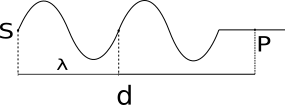
\includegraphics{EtudeMathOndeSinusProg.png}
\end{center}
P fait la même chose que S avec avec un retard qui correspond au temps mis pour arriver à P.
\begin{equation}
    \begin{split}
        y_{P(t)} & = A \cdot sin(\omega t + \phi) \\
        &= A \cdot sin(\omega (t-t')) \text{ où } t' = \dfrac{d}{v}\\
        &= A\cdot sin\Big(\omega t - \omega \dfrac{d}{v}\Big)\\
        &= A \cdot sin\Big(\omega t - \dfrac{2\pi}{T}\cdot \dfrac{d}{v}\Big) \\
        &= A \cdot sin\Big(\omega t - \dfrac{2\pi d}{\lambda}\Big) \text{ valable pour } t > t'
    \end{split}
\end{equation}
Conditions pour que P et S vibrent en concodrance de phase.
\begin{equation}
    \begin{split}
        y_{S(t)} &= y_{P(t)}  \text{ et même v}\\
        A\cdot sin(\omega t) &= A\cdot sin\Big(\omega t - \dfrac{2\pi d}{\lambda}\Big)\\
         sin(\omega t) &= sin\Big(\omega t - \dfrac{2\pi d}{\lambda}\Big)\\
         \omega t &= \omega t - \dfrac{2\pi d}{\lambda} + k2\pi \\
         0 &=  - \dfrac{2\pi d}{\lambda} + k2\pi \\
         k2\pi &= \dfrac{2\pi d}{\lambda} \\
         k\cdot \lambda& = d \text{  } k \in \mathbb{N}
    \end{split}
\end{equation}
Conditions pour que S et P soient en oppositions de phase.
\begin{equation}
    \begin{split}
        y_{S(t)} &= -y_{P(t)}\\
        A\cdot sin(\omega t) &= -A \cdot sin\Big(\omega t - \dfrac{2\pi d}{\lambda}\Big)\\
        \omega t &= \omega t - \dfrac{2\pi d}{\lambda} + \pi + k2\pi\\
        \dfrac{2\pi d}{\lambda}& = \pi + k2\pi\\
        \dfrac{2 d}{\lambda}& = 1+2k\\
        d&= (2k+1)\cdot \dfrac{\lambda}{2} \text{ } k \in \mathbb{N}\\
    \end{split}
\end{equation}

\subsubsection{Vitesses des ondes progressives le long d'une corde}
Dans un référentiel qui se déplace avec l'onde, c'est la corde qui se déplace vers la gauche.
\begin{center}
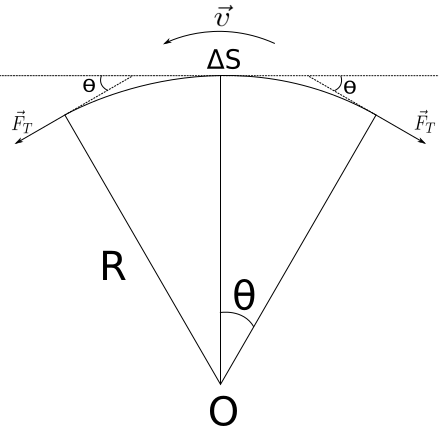
\includegraphics[scale = 0.75]{vitesseOndeProgCord.png}\\
\end{center}
Un petit segment de corde $\Delta S$ peut être assimilé à un arc de cercle.
\begin{equation}
    \Delta S = R(2 \theta)
\end{equation}
Si $\mu$ est la densité de masse linéique (la masse par mètre (kg/m)), la masse du segment est:
\begin{equation}
    m=\mu \Delta S= \mu R(2\theta)
\end{equation}
La tension de la corde doit fournir la force centripète nécessaire au mouvement circulaire.
\begin{equation}
    \begin{split}
        2F_T \cdot sin(\theta) &= \dfrac{mv^2}{R}
    \end{split}
\end{equation}
Si l'amplitude de la déformation est petite, $sin(\theta)\cong \theta$, alors,
\begin{equation}
    \begin{split}
        2F_T \cdot sin(\theta) &=  2\mu R \theta \cdot \dfrac{v^2}{R}\\
        v &= \sqrt{\dfrac{F_T}{\mu}}
    \end{split}
\end{equation}

\section{Propagation des ondes à deux dimensions}
\subsection{Propagation sans obstacles}
\subsubsection{Observations}
\begin{enumerate}
    \item Ondes circulaires\\
    En chacun des points, la direction de propagation de ces ondes circulaires est radiale, c'est-à-dire perpendiculaire aux circonférences.\\
    L'amplitude diminue en fonction du temps. Au plus le temps s'écoule, le diametre du cercle augmente donc le périmètre augmente. L'énergie est donc répartie sur toute la longeur du périmètre.
    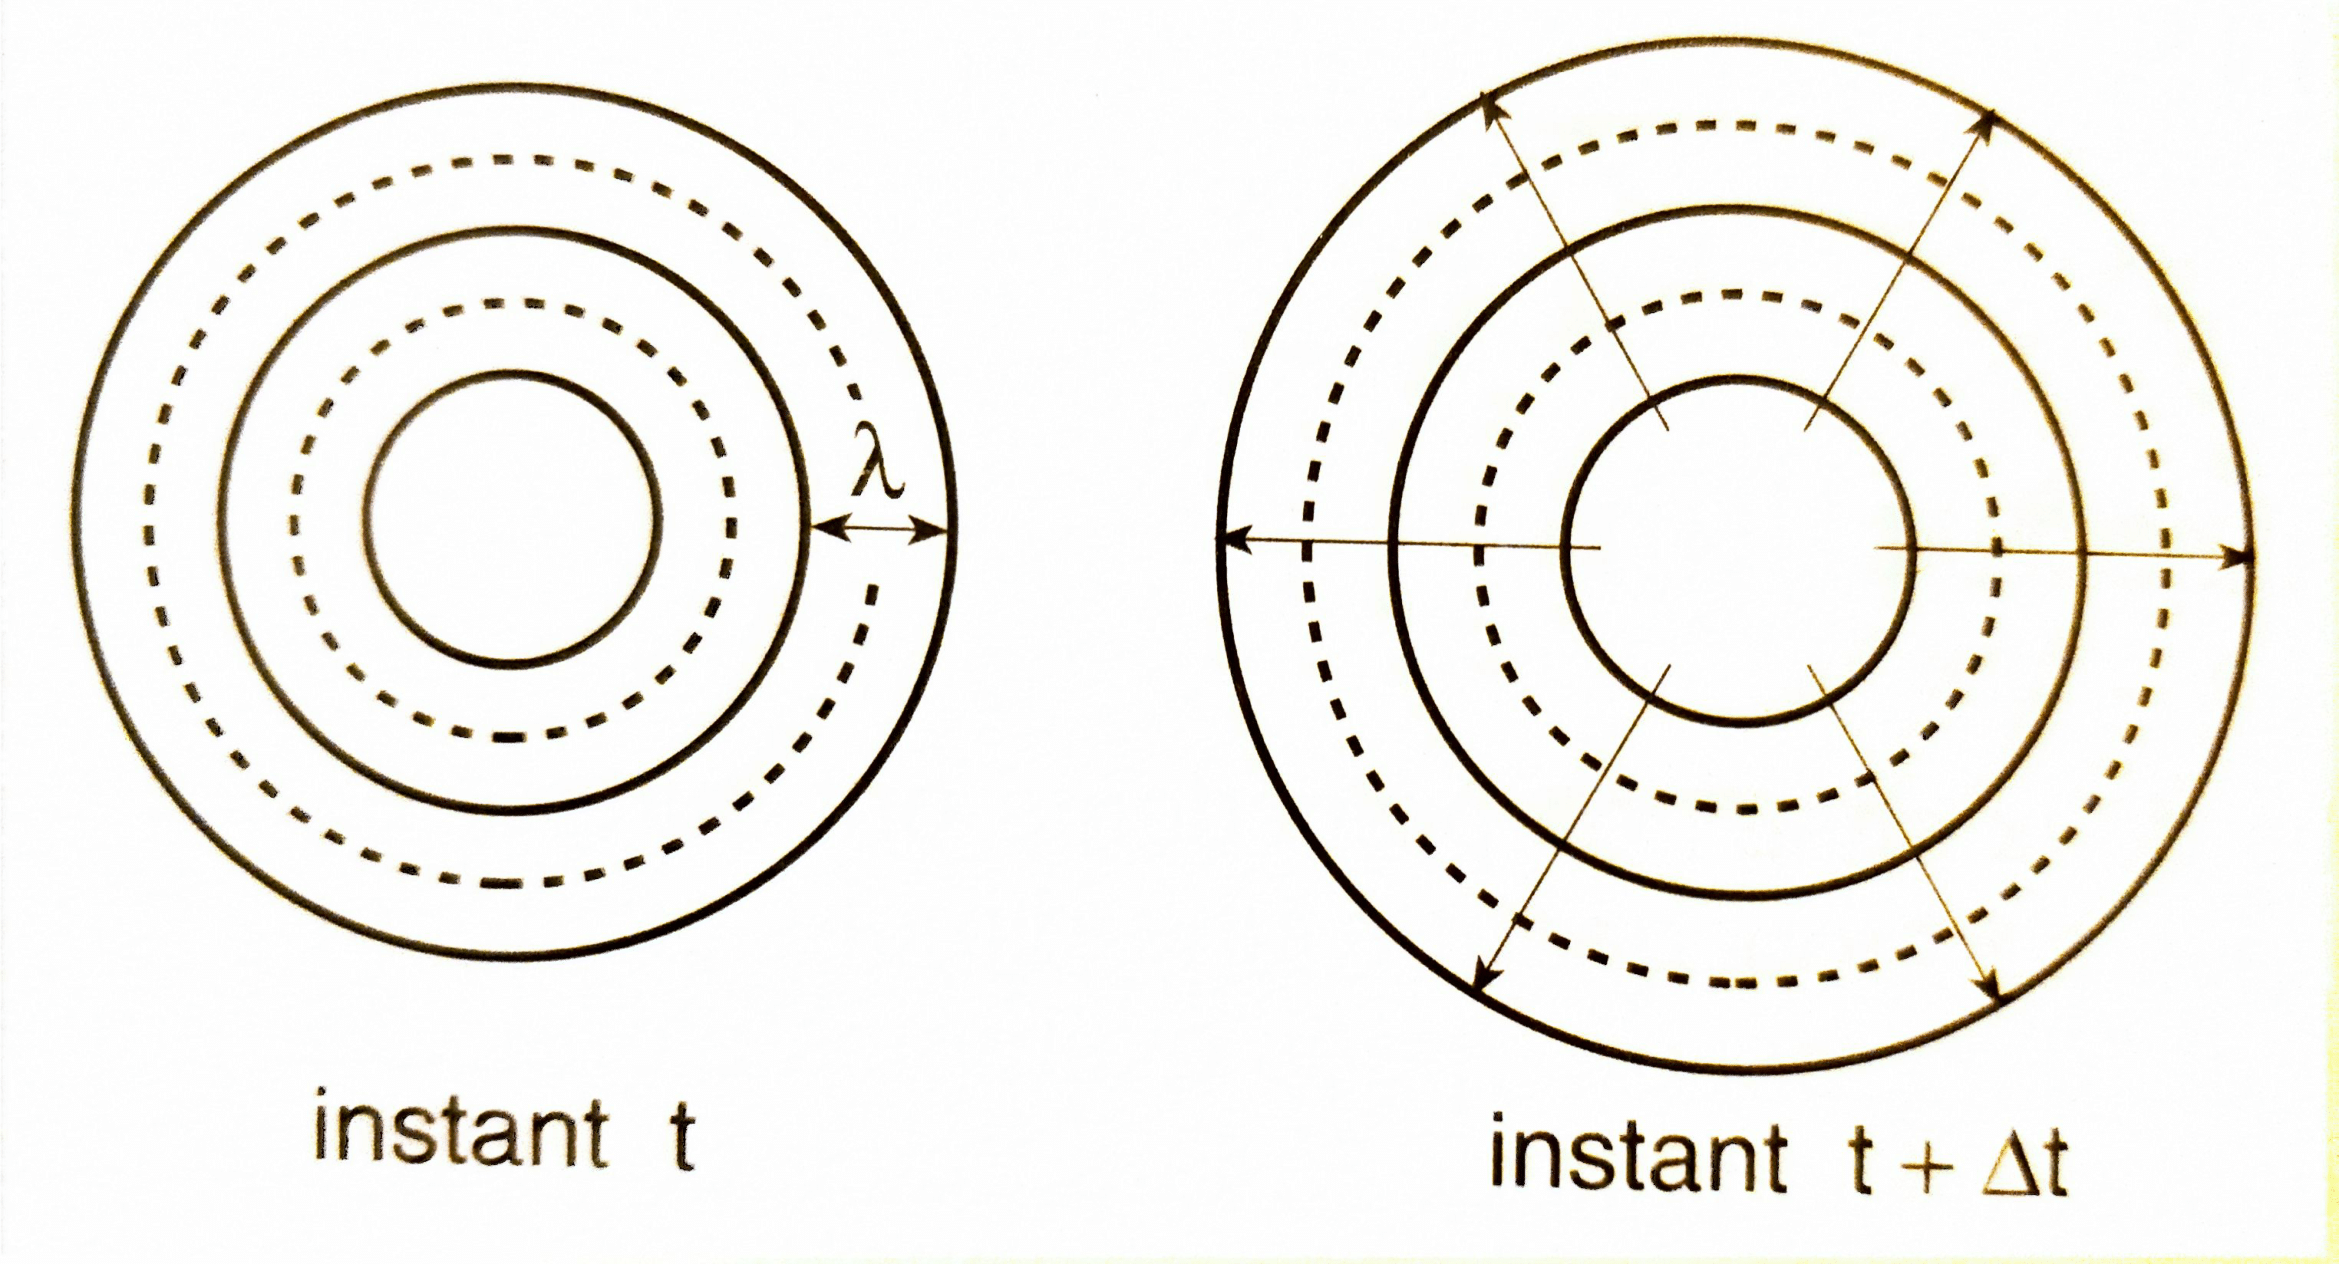
\includegraphics[scale = 0.1]{OndesCirculairesPropag.png}
    \item Ondes planes\\
    La direction de propagation est perpendiculaire aux crêtes.
    \item Conclusion.\\
    Les ondes se propagent en ligne droite.
\end{enumerate}
\subsubsection{Principe de Huygens}
Tout point atteint par une onde se comporte comme une source d'ondes, c'est-à-dire génère des ondes élémentaires circulaires de même fréquences.
\begin{itemize}
    \item Le principe de Huygens permet donc de prévoir qu'une onde circulaire va se propager en restant une onde circulaire.
    \item Le principe de Huygens permet donc de prévoir qu'une onde plane se propage en restant une onde plane.
\end{itemize}
\subsection{Réflexion des ondes}
\subsubsection{Observations}
\begin{enumerate}
    \item Ondes circulaires\\
    Voir illustrations 4.7 p.49
    \item Ondes planes\\
    Voir illustrations 4.8 p.50
\end{enumerate}
\subsection{Réfraction des ondes}
Les ondes ne se propagent pas à la même vitesse dans des milieux différents.
\subsubsection{Explications théoriques}
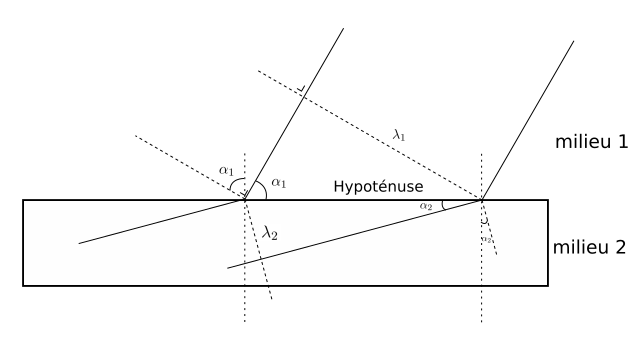
\includegraphics[scale=0.5]{DemonstrationRefraction.png}\\
\begin{align}
    \systeme*{sin\alpha_1 &= \dfrac{\lambda_1}{hyp},sin\alpha_2 &= \dfrac{\lambda_2}{hyp}}\Longrightarrow
    \dfrac{sin\alpha_1}{sin\alpha_2} = \dfrac{\lambda_1}{\lambda_2} =\dfrac{v_1\cdot T}{v_2\cdot T} =\dfrac{v_1}{v_2}
\end{align}

\subsection{Diffraction des ondes}
\subsubsection{Observations}
L'orsque l'écart = la longeur d'onde. L'onde se réfracte.\\
Au plus on réduit la distance, au plus la difraction est forte.
\subsubsection{Synthèse}
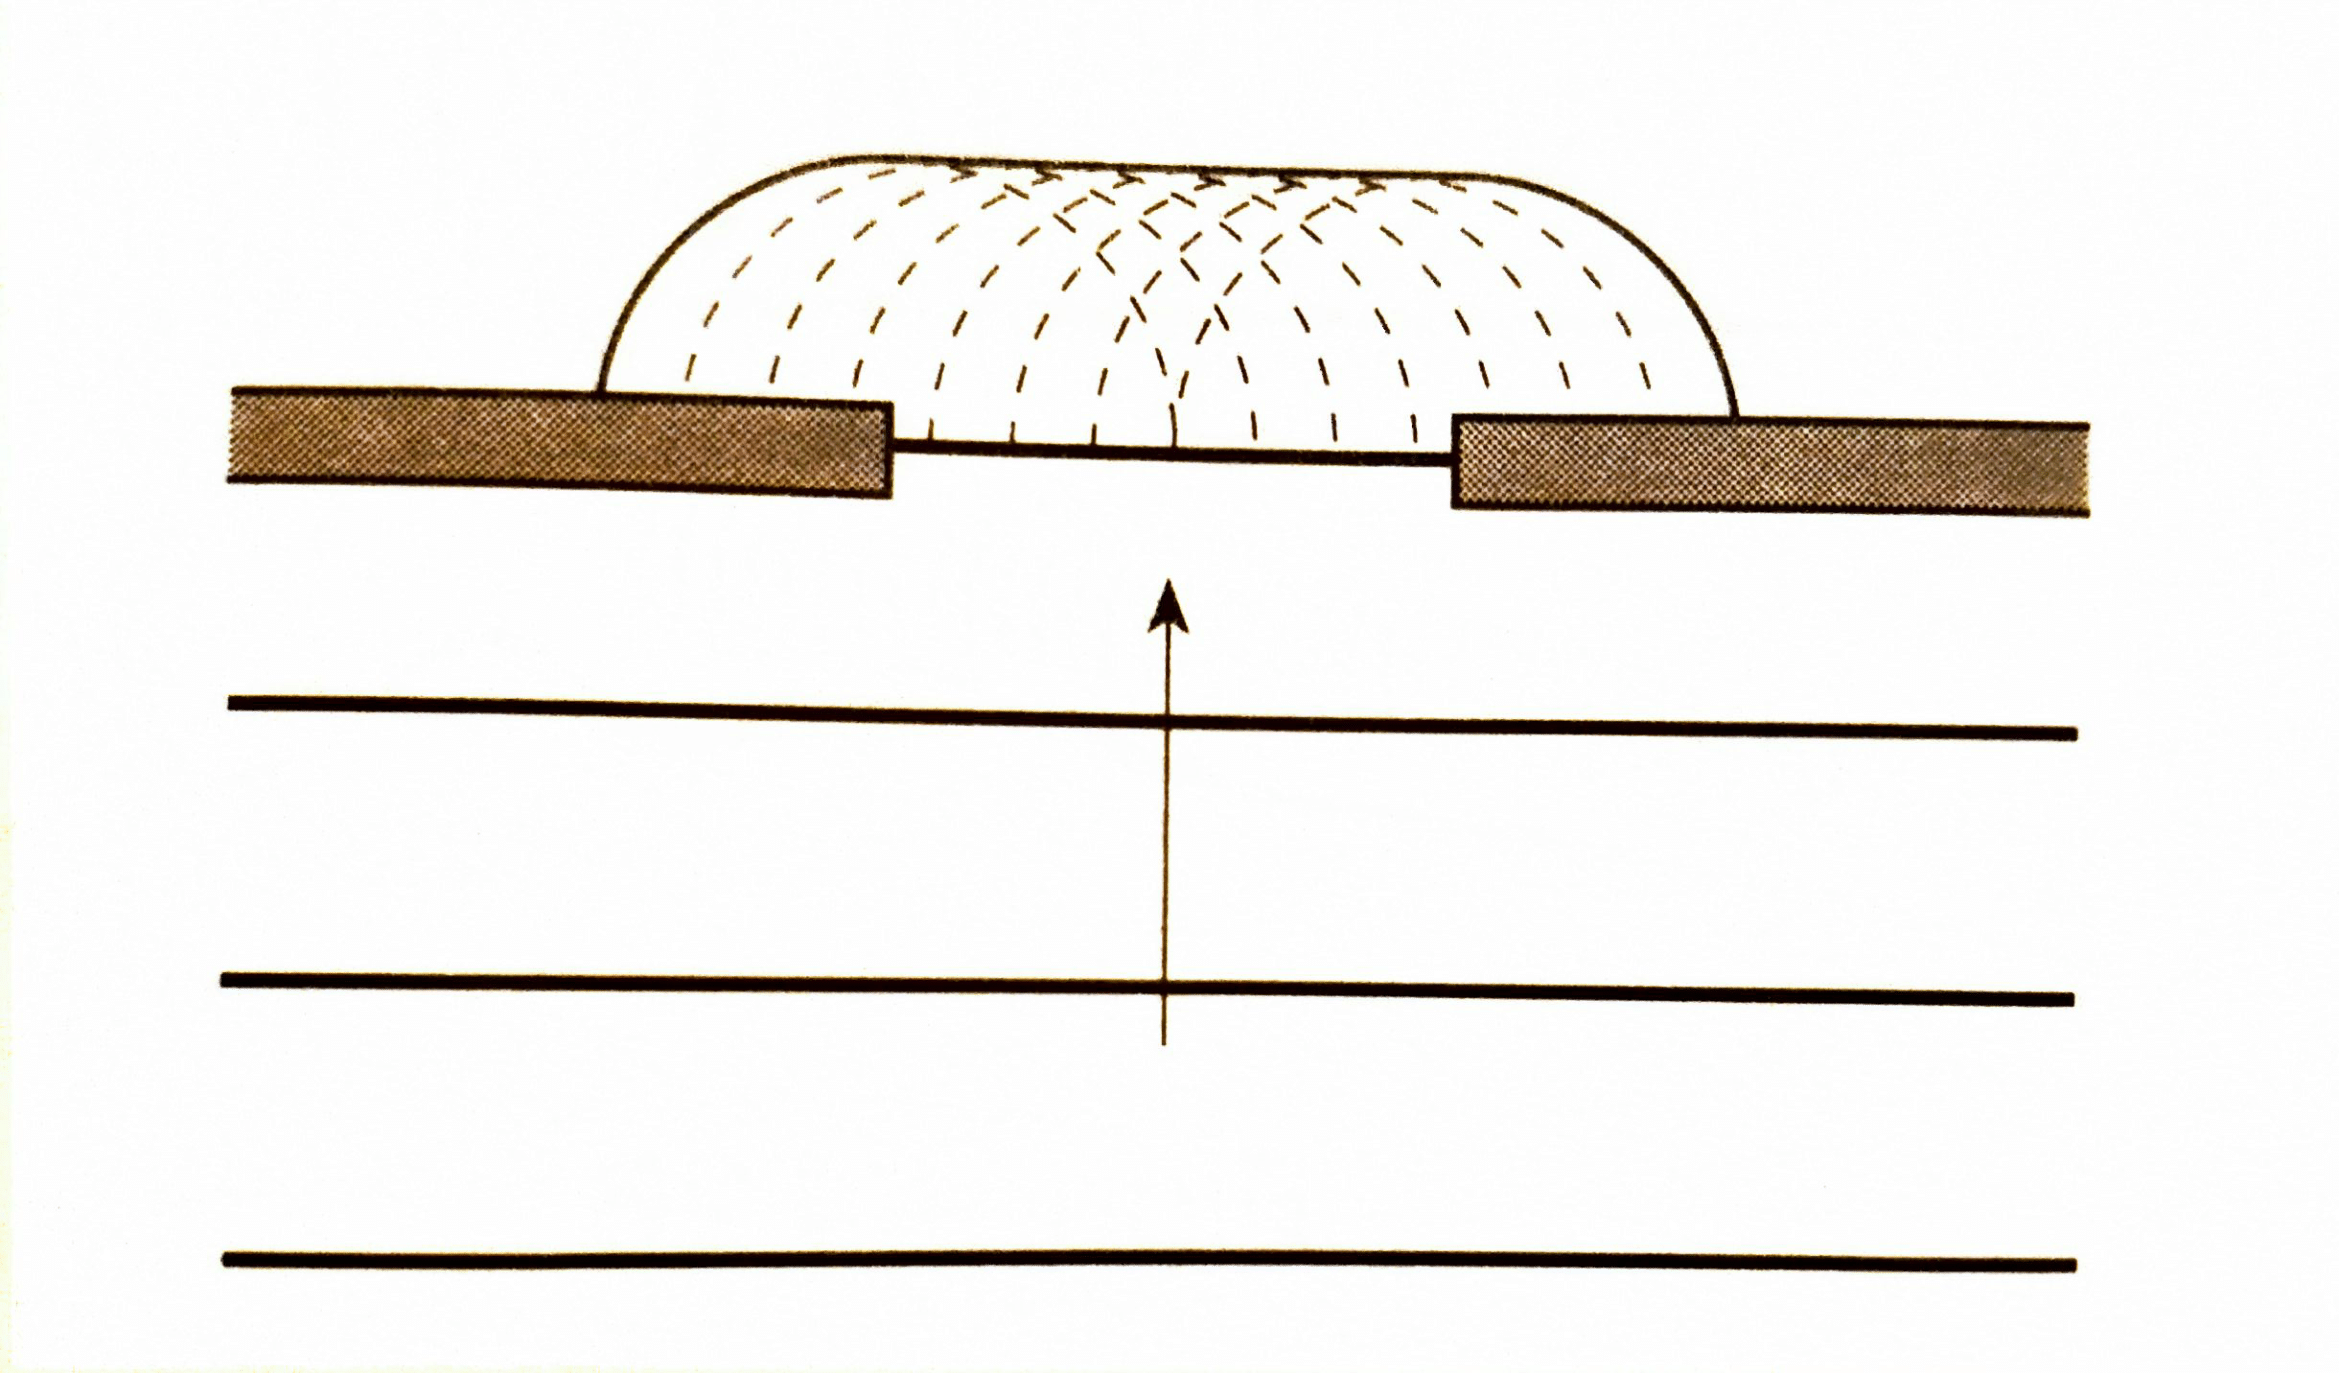
\includegraphics[scale=0.1]{DiffractionOndes.png}\\

La diffraction des ondes est leur déviation dans plusieurs directions par des obstacles: elles sont déviées de leur direction initiale.\\
Elles ne se propagent plus en ligne droite.\\
Lorsque que la longeur d'onde est infieure à la largeur de l'obstacle. Il n'y a pas de phénomène de diffraction. L'onde continue en ligne droite.\\
Lorsque la longeur d'onde se rapproche de la largeur de l'obstacle, il y a de plus en plus un phénomène de réfraction.\\
Lorsque la longeur d'onde est égale ou supérieur à la largeur de l'obstacle, il y a beaucoup de diffraction.


\section{Superposition d'ondes}
\subsection{Principes de superposition}
Les différentes ondes ne changent pas. Elles ne s'altèrent pas entre elles.
\subsubsection{Conclusion}
L'élongation en un point, à un instant donné, est la somme algébrique des élongations en ce point de chacune de ces pertubations à cet instant.\\
\begin{align}
    y(t)&=y_1(t)+y_2(t)\\
    y&=\sum y_i
\end{align}
Après la rencontre, les perturbations continuent à se propager indépendamment l'une de l'autre dans leur sens initial.
\subsection{Modes stationnaires d'oscillation}
\subsubsection{Etude graphique}
Endroits où les ondes sont toujours en opposition de phase: noeud\\
Nedroits où les ondes sont toujours en concordance de phase: ventre
\end{document}
